\documentclass[a4paper,10pt]{article}
\usepackage[utf8]{inputenc}
\usepackage{lipsum}
\usepackage[section]{placeins}
\usepackage{listings,xcolor}
\usepackage{enumerate}
\usepackage{booktabs}
\usepackage{vhistory}
\usepackage{graphicx}
\usepackage{placeins}
\usepackage{float}
\usepackage{rotating}
\usepackage{afterpage}
\usepackage{color}
\usepackage[showframe=false]{geometry}
\usepackage{changepage}
\setcounter{tocdepth}{3}
\setcounter{secnumdepth}{3}
\title{Integration Testing Plan Document}
\author{Joan Ficapal Vila (876805), Nicolò Vendramin (879113)}
\date{\today\\v1.0}
\begin{document}
  \pagenumbering{Roman}
  \begin{figure}[t]
  \centering
    
\includegraphics[scale=0.3]{Resources/logoPolimi.png}
  \end{figure}
  \thispagestyle{empty}
  \maketitle
  \newpage
  \begin{versionhistory}
    \vhEntry{0.1}{01.01.17}{N and J}{Initiated the document}
    \vhEntry{0.2}{04.01.17}{N and J}{Wrote the introduction}
    \vhEntry{0.3}{08.01.17}{N and J}{Defined the Integration Strategy}
    \vhEntry{0.4}{10.01.17}{N}{Graphs of the Second Section}
    \vhEntry{0.5}{11.01.17}{N and J}{Started working on the tables}
    \vhEntry{0.6}{12.01.17}{J}{Added tests to the Tables}
    \vhEntry{0.7}{13.01.17}{N and J}{Added tests to the Tables}
    \vhEntry{0.8}{14.01.17}{N}{Wrote the final Section}
    \vhEntry{1.0}{15.01.17}{N and J}{First Release}
    
 
    
  \end{versionhistory}
  \paragraph{Hours of work}
  \begin{description}
    \item[$\bullet$] Joan Ficapal Vila : 10 hours
    \item[$\bullet$] Nicolò Vendramin : 10 hours
   \end{description}
   \newpage
  \tableofcontents
  \newpage
  \pagenumbering{arabic}

\maketitle
\section{Introduction}
\subsection{Purpose and Scope}
\paragraph{} This document is the Integration Testing Plan Document for the PowerEnjoy application. \\ It is produced in order to specify in detail how
the testing process must be performed in order to guarantee a correct and deep analysis of the application's behaviour.\\ Integration testing must be considered a key 
activity in order to ensure the correct functioning of the cohoperation between all the subsystems composing the software to be developed. As a matter of fact the unit testing itself is not 
sufficient to make sure that the overall system in its complex works as established. \\
\paragraph{}To outline in a clear way the main aspects concerning this part of the testing activity we are going to include in this document, in a precise but concise way, the following informations:
  \begin{description}
    \item[$\bullet$] Description of the components that must go through integration testing
    \item[$\bullet$] The integration strategy to be followed during the testing activity
    \item[$\bullet$] The precedences to be followed during the process
    \item[$\bullet$] A description of the testing activities including the input and the expected effect for the more relevant parts
    \item[$\bullet$] An outline of the tools and equipments needed.
  \end{description}
\subsection{Definitions, Acronyms and Abbreviations}
  \subsubsection{Acronyms}
  \begin{description}
    \item[$\bullet$] \textbf{API:} Access point of Interface. This term is used to indicate the interfaces exposed to access a software
    service from another software service.
    \item[$\bullet$] \textbf{DD:} Design Document. This document.
    \item[$\bullet$] \textbf{RASD:} Requirements Analysis and Specifications Document. The reference document for the specifications of the system to be developed.
    \item[$\bullet$] \textbf{DAG:} Direct Acyclic Graph. A DAG is a graph made up of nodes and directed archs in which no cycles are present.
  \end{description}
  \subsubsection{Definitions}
   \begin{description}
   \item[$\bullet$] \textbf{Unit Testing:} With unit testing is meant that activity that make sure that every basic unit that composes the software is correctly 
   working as expected. With unit we indicate the smaller atom of which the software is composed. In case of a Java program we can assume Classes as units.
   \item[$\bullet$] \textbf{Integration Testing:} With integration testing is meant that phase 
   of software testing in which individual modules are tested together as a group.
   \end{description}
\subsection{Reference Documents}
Here we attached the list of all the documents that are kept as references in the writing of this document.
\begin{description}
    \item[$\bullet$] PowerEnjoy RASD Document.
    \item[$\bullet$] PowerEnjoy Design Document.
    \item[$\bullet$] Course Slides.
    \item[$\bullet$] Templates provided at lesson.
  \end{description}
 \newpage
 
\section{Integration Strategy}
\subsection{Entry Criteria}
In order to ensure that the testing process is completed with good results some conditions must to be met. At first is required that both the RASD and the DD are 
completed and defined. This condition must be guaranteed to have a complete and detailed description of the system requirements and 
design on which to base the testing activities. \\
In addition before to start the very integration process it is required to pass the single components of the system with unit testing. It's important that before integrating 
two components each of them have passed all the unit tests that were designed for them. We assume that for the components included in the request manager and controller
the percentage of coverage reached before starting their integration is between 95\% and 100\%.
For what the Client Application is concerned, since it's a graphical interface, the unit testing needed before the integration should be at least 70\%; making sure that 
the only non tested components are the parts related to the very presentation and not the ones related to the data exchange process.
\\An additional condition that must be met before starting the integration testing activity is that the functioning of all the API has been checked to be as expected from
the documentation. In order to meet this hypothesis a detailed checking activity must be done in order 
to verify the behaviour of the APIs provided by the external services used. 
in the software.
\subsection{Elements to be integrated} Since a precise description of all the components is given in the DD we invite the reader to refer to that document in case of need.\\
The integration testing is made in order to verify the joint operation of the following group of components. \\
As stated before we assume that all the components belonging to the following list, before being integrated
satisfy the unit level coverage specified in the previous paragraph. The unit to integrate are:
\begin{description}
    \item[$\bullet$] Mobile Client
    \item[$\bullet$] Request Manager
    \item[$\bullet$] Controller
\begin{description}
    \item[$\circ$] Registration and Login Manager
    \item[$\circ$] Pricing and Discount Manager
    \item[$\circ$] Service Manager
    \item[$\circ$] Resource Manager
  \end{description}
  \end{description}
\subsection{Integration Testing Strategy} To design the strategy to be used for the integration testing
we took into account different factors among which the more importants are the architectural structure of the software
described in the DD and the willing to optimize the work during the testing process.\\ The best solution identified
to fit the above mentioned needs is to adopt a Bottom-Up and Core-module-first approach. In practical terms this means that at first
we are going to integrate the low level components between them and only after that we
will test the communication between the high level components. The core-module-first approach means
that we will give a major priority to the integration of those components that form the controller system in order
to be sure that all the core functionalities of the application are provided in the correct way and that the controller
works as an integrated system.\\
At the end of the integration testing we allocate some human resources to the further verification through usage of the system.
For this final verification activity we don't give precise indication and we invite the dedicated staff to follow the possible
use cases outlined in the DD, and to repeatedly test them in different environmental conditions,
and following the different possible branches described in the 
use cases' tables making sure to cover, as much as possible, both exceptional and non-exceptional behaviours of the system.
\subsection{Sequence of component/ function integration}
\subsubsection{Subsystem 1}
\begin{description}
    \item[$\bullet$] I1. Resource Manager $\rightarrow$ DBMS
    \item[$\bullet$] I2. Registration / Login Manager $\rightarrow$ Existing System
    \item[$\bullet$] I3. Registration / Login Manager $\rightarrow$ Resource Manager
    \item[$\bullet$] I4. Service Manager $\rightarrow$ Existing System
    \item[$\bullet$] I5. Service Manager $\rightarrow$ Resource Manager
    \item[$\bullet$] I6. Service Manager $\rightarrow$ Registration / Login Manager
    \item[$\bullet$] I7. Price and Discount Manager $\rightarrow$ Billing System
    \item[$\bullet$] I8. Price and Discount Manager $\rightarrow$ Resource Manager
    \item[$\bullet$] I9. Service Manager $\rightarrow$ Price and Discount Manager
  \end{description}
  \begin{figure}[!h]
  \centering
    \includegraphics[scale=0.50]{Resources/subsistem1.png}
    \caption{Subsystem 1, Integration Strategy}
  \end{figure}
  \FloatBarrier
  \subsubsection{Subsystem 2}
\begin{description}
    \item[$\bullet$] I10. BookVehicle, CancelBooking, OpenVehicle, Conclude $\rightarrow$ Service Manager
    \item[$\bullet$] I11. Login, Logout, Register $\rightarrow$ Registration / Log in Manager
    \item[$\bullet$] I12. ShowVehicles, ShowCarDetails, ShowAccountInfo $\rightarrow$ Resource Manager
  \end{description}
  \begin{figure}[!h]
  \centering
    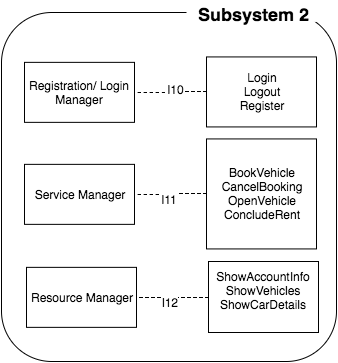
\includegraphics[scale=0.50]{Resources/subsistem2.png}
    \caption{Subsystem 2, Integration Strategy}
  \end{figure}
  \FloatBarrier
 \subsubsection{Subsystem 3}
\begin{description}
    \item[$\bullet$] I12. Mobile Client $\rightarrow$ Request Manager
  \end{description}
  \begin{figure}[!h]
  \centering
    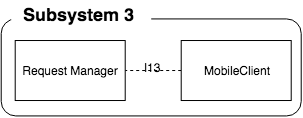
\includegraphics[scale=0.50]{Resources/subsistem3.png}
    \caption{Subsystem 3, Integration Strategy}
  \end{figure}
  \FloatBarrier
\subsection{Further Conisderation On The Sequence of Integration}
Before concluding the section about the integration strategy we attach the direct acyclic graph of the dependencies between the different
integrations steps. This is provided
for two basics reasons: 
\begin{description}
    \item[$\bullet$] to provide a further check that all the components are integrated in a correct sequence 
    \item[$\bullet$] if in case of need the integration strategy cannot be followed as above, or it is more efficient to change it, 
the DAG must be kept as a reference
and the new strategy should ensure that all the dependencies are managed as specified by the graph.
  \end{description}
  \begin{figure}[!h]
  \centering
    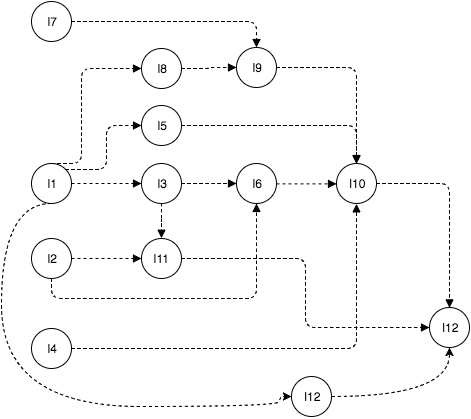
\includegraphics[scale=0.8]{Resources/dagdependencies.png}
    \caption{Direct Acyclic Graph of Integration Dependencies}
  \end{figure}
  \clearpage
\section{Individual Steps and Test Description}
  \begin{figure}[!h]
  \centering
    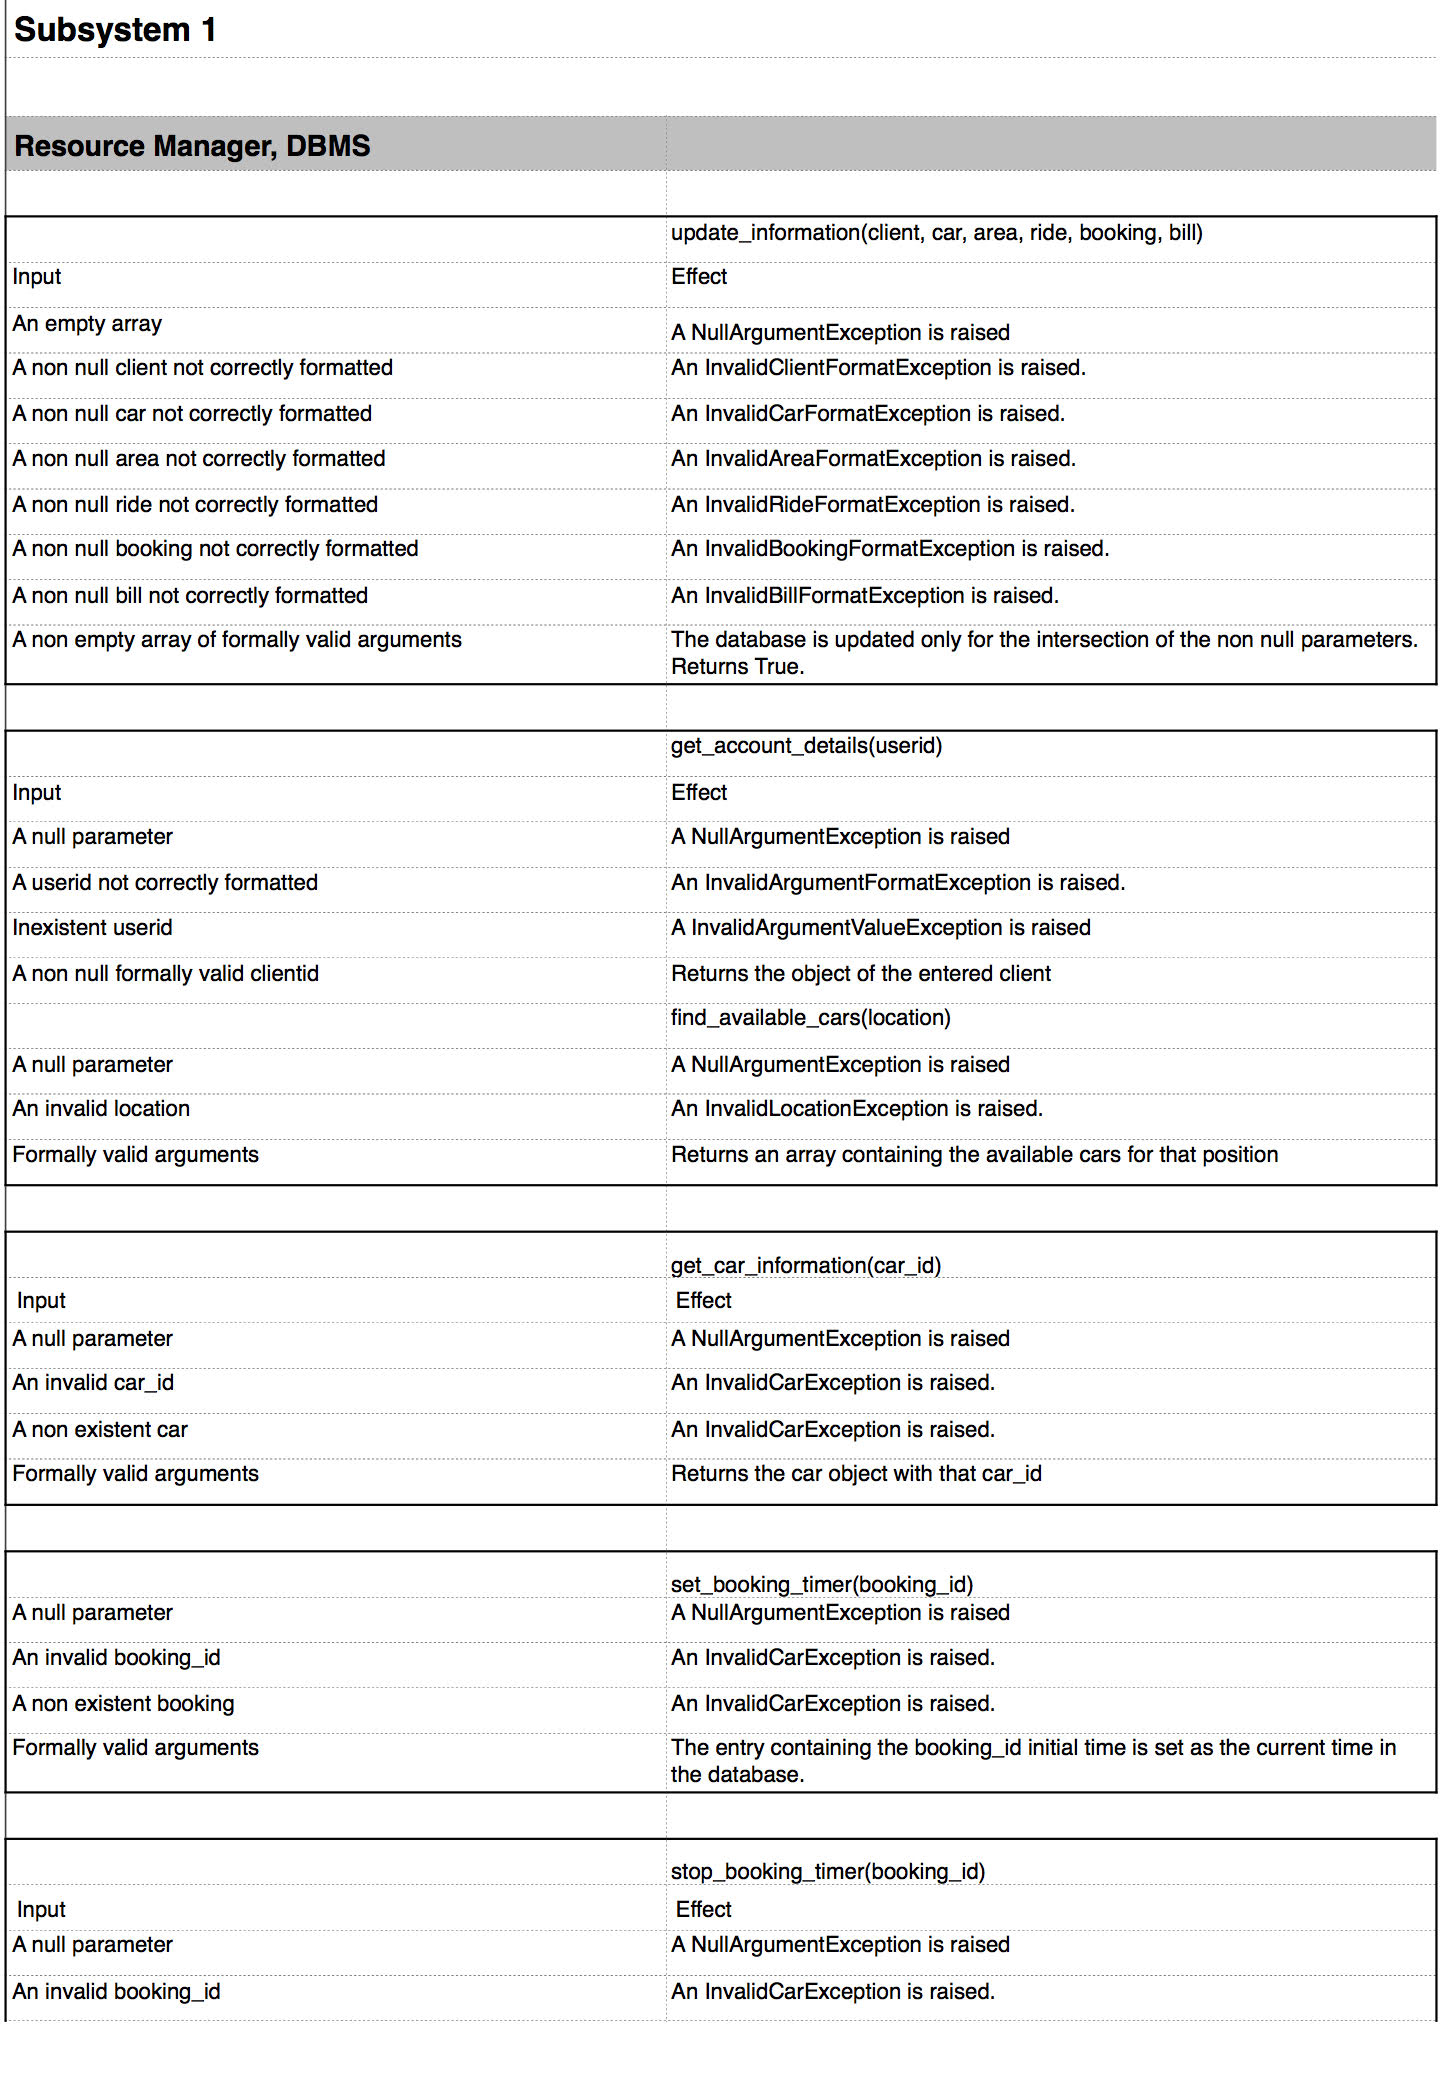
\includegraphics[scale=0.26]{Resources/1.jpg}
  \end{figure}
    \begin{figure}[!h]
  \centering
    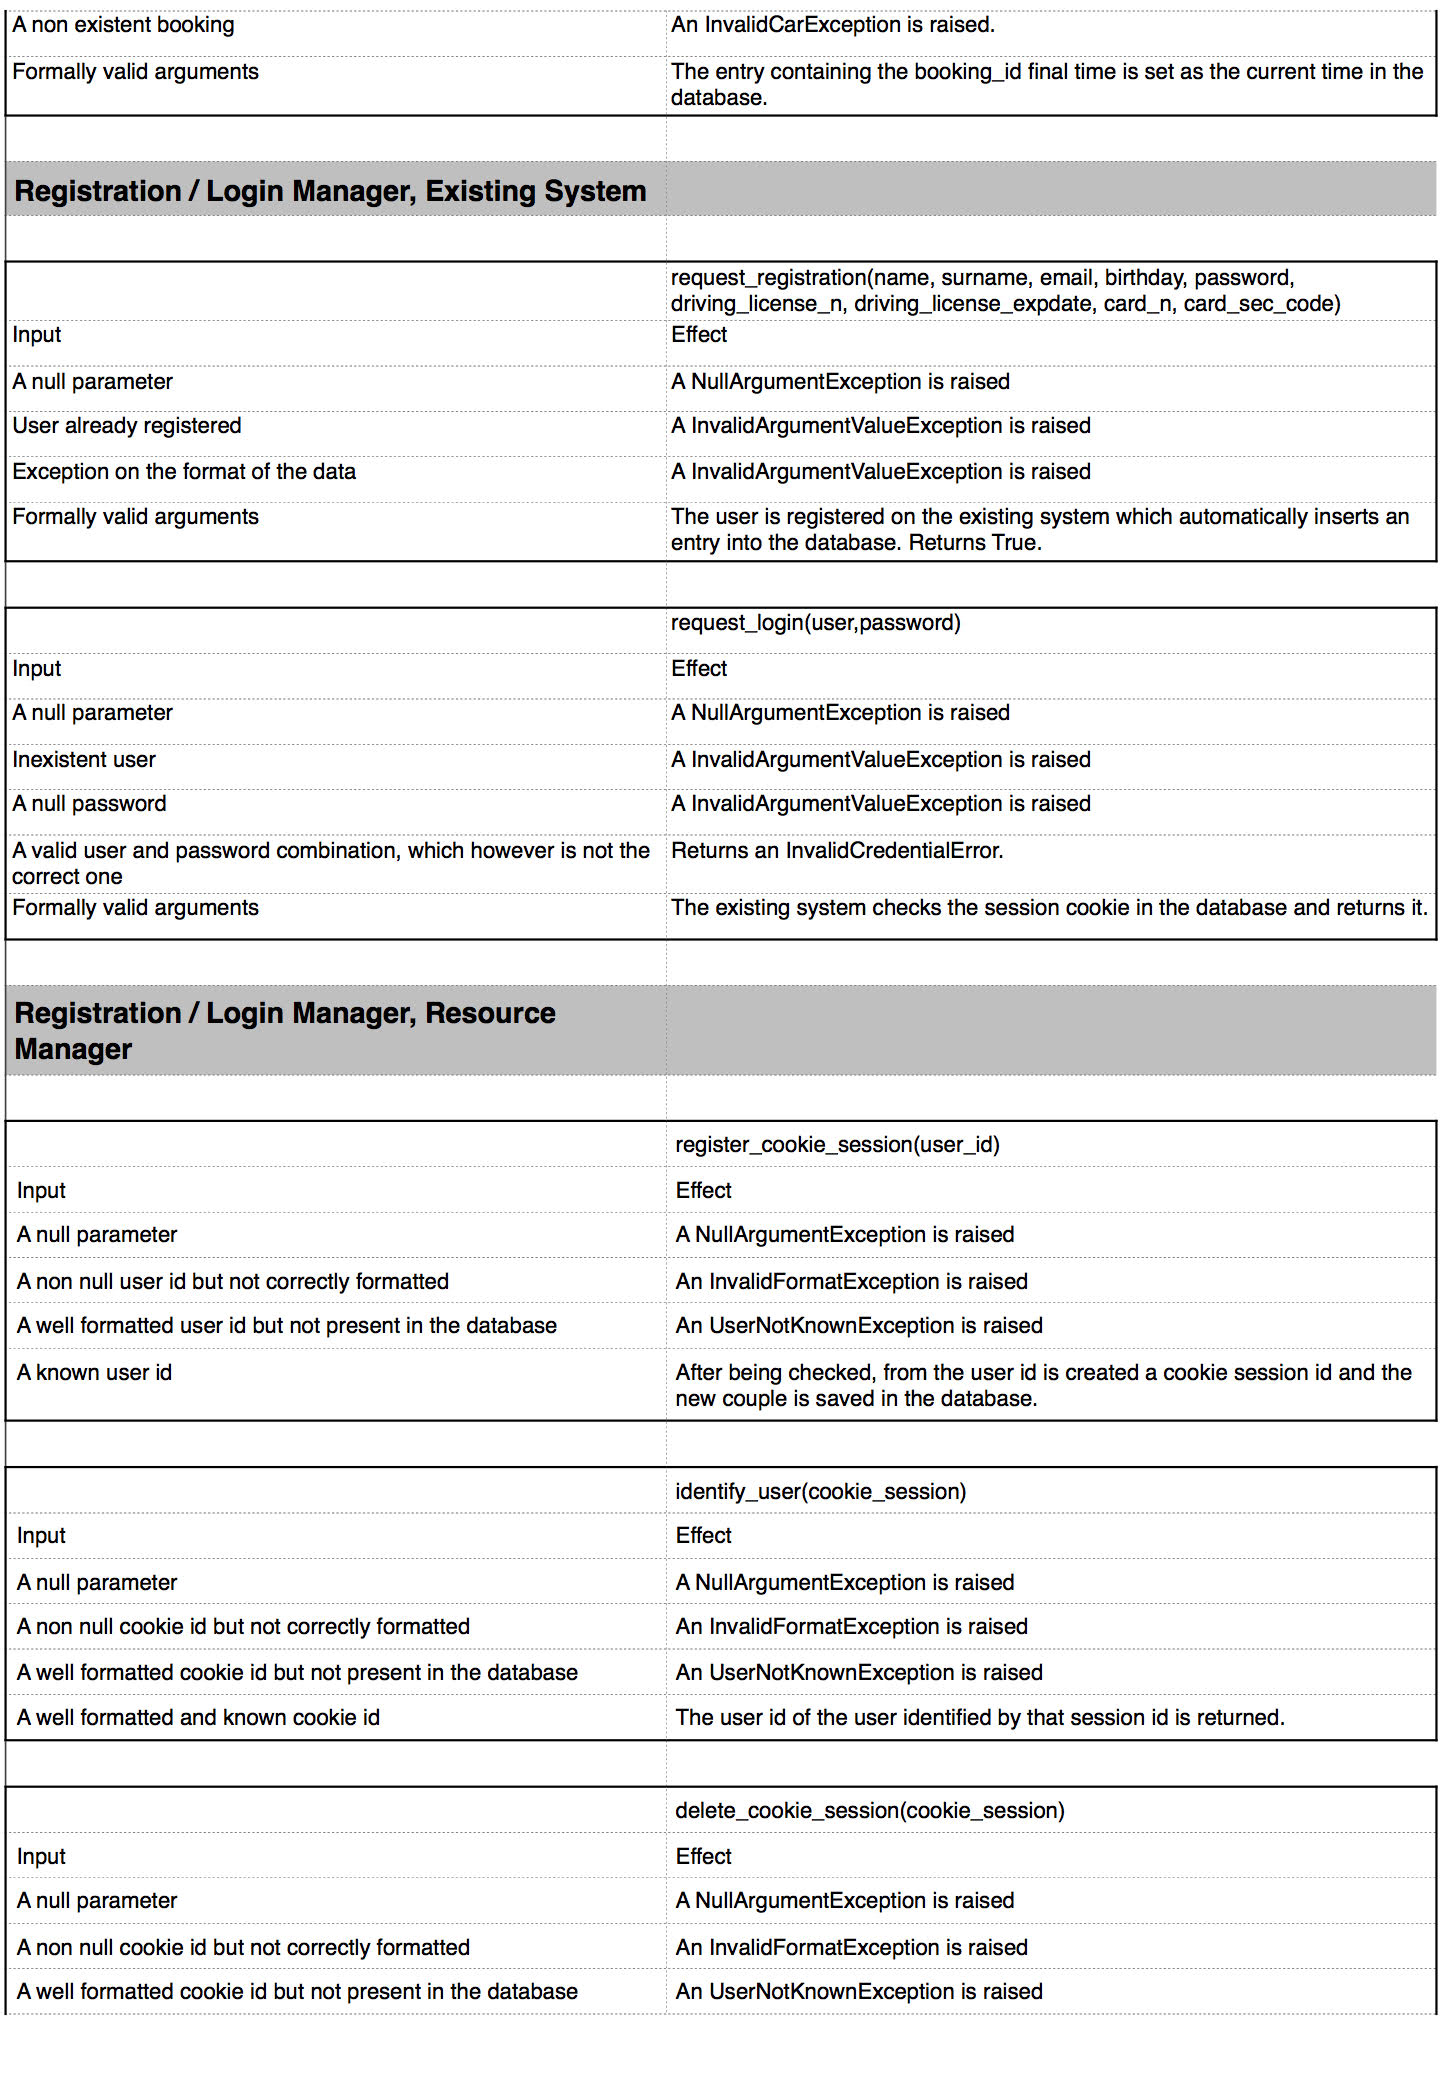
\includegraphics[scale=0.26]{Resources/2.jpg}
  \end{figure}
    \begin{figure}[!h]
  \centering
    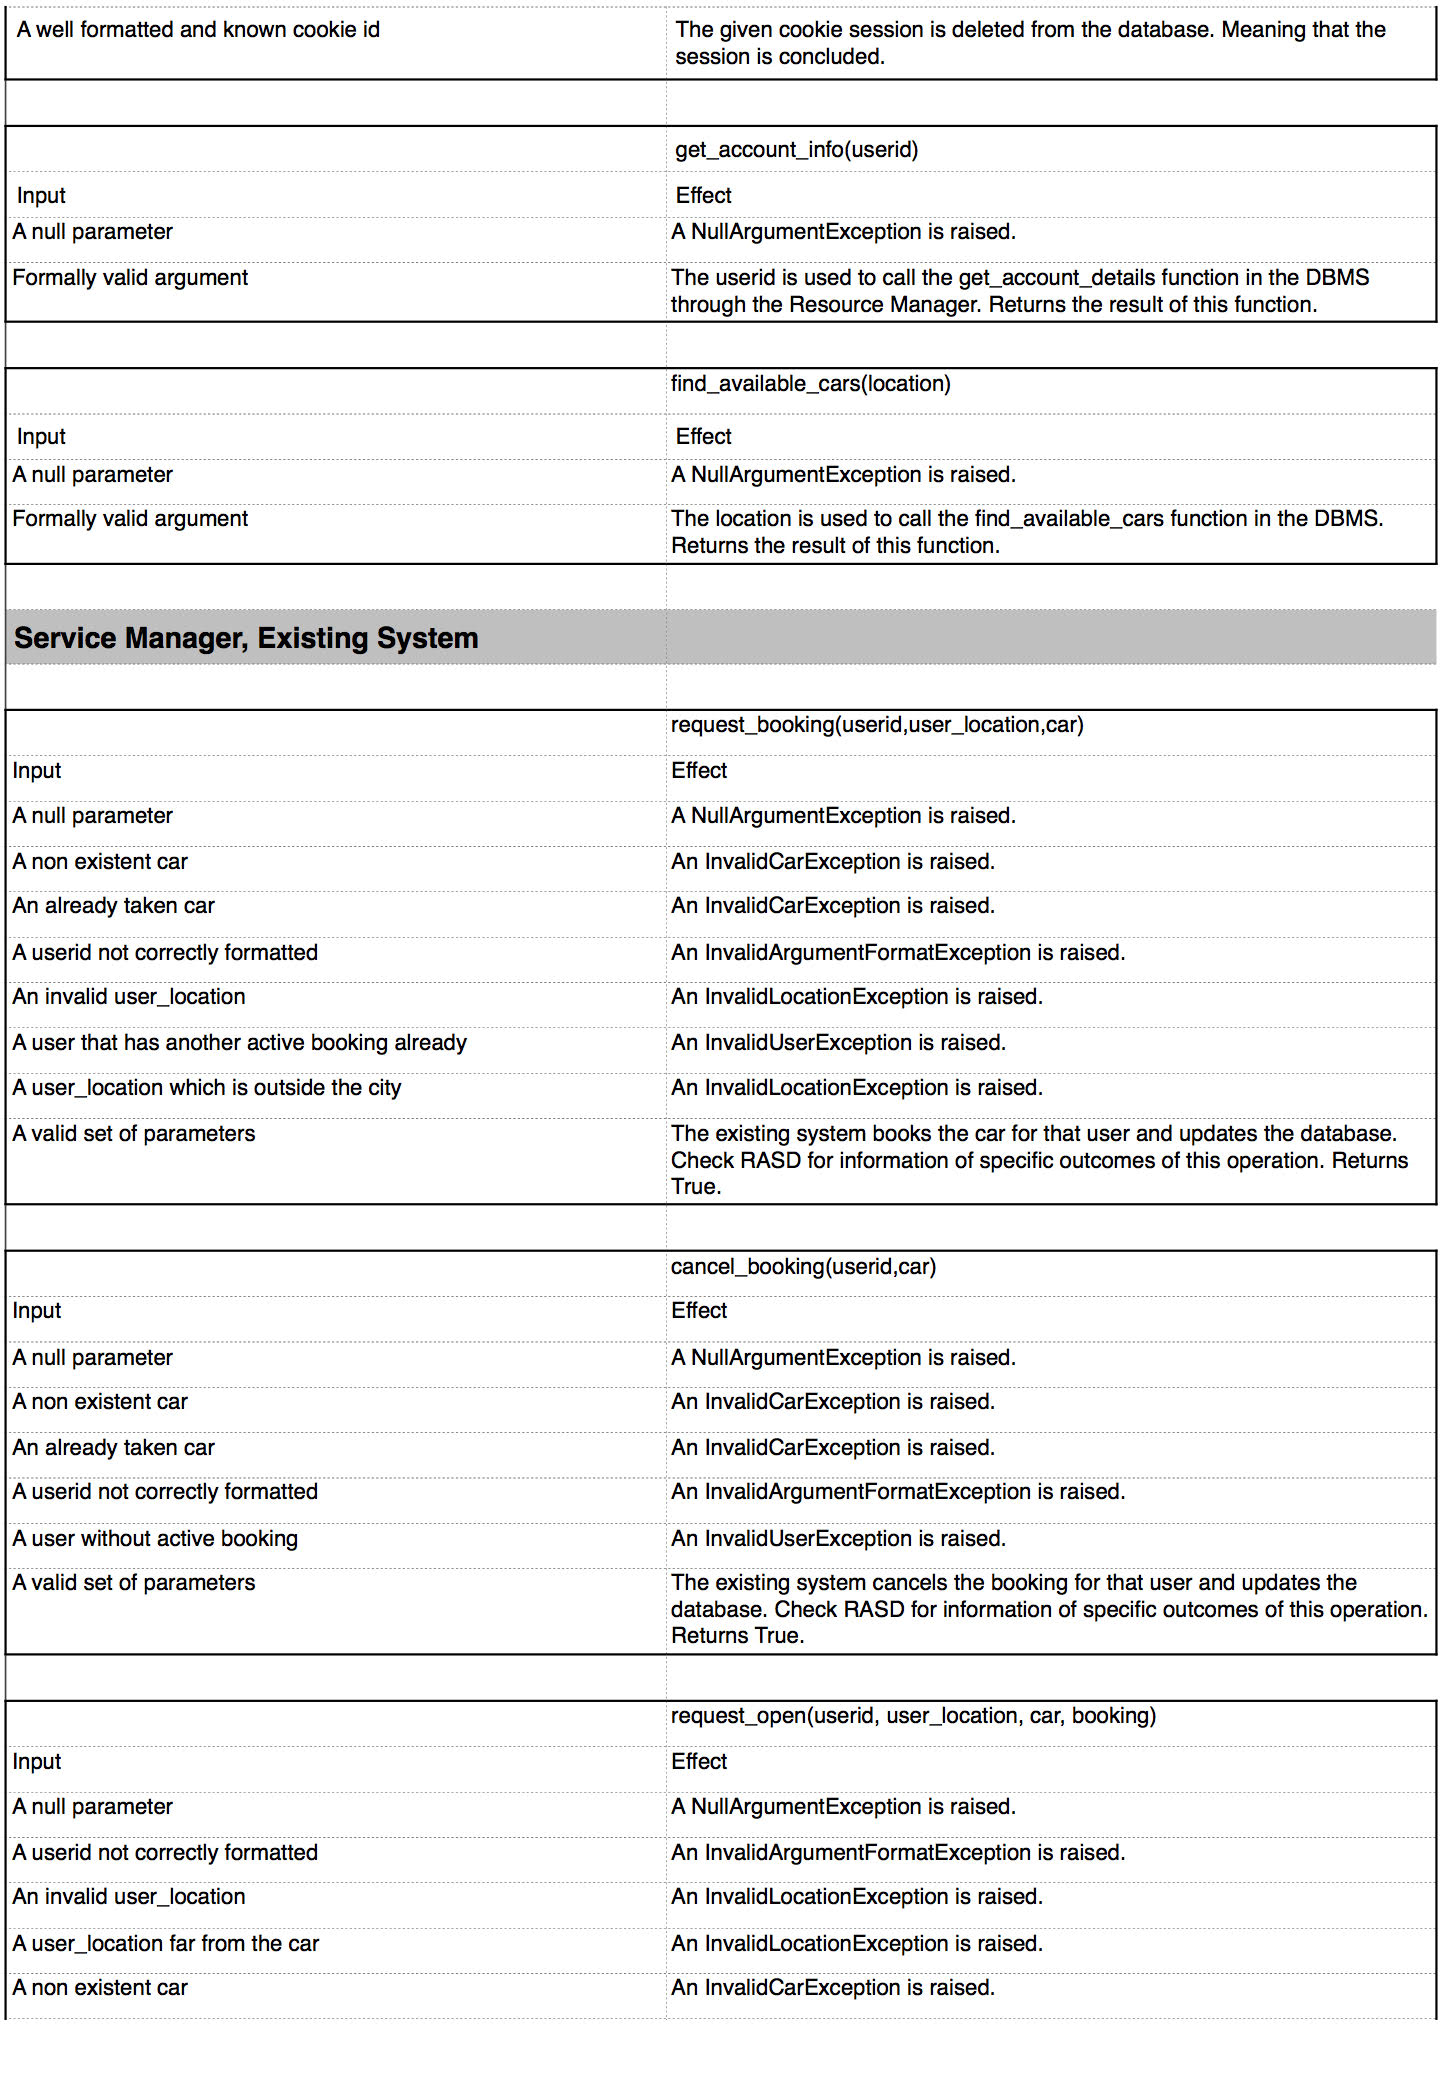
\includegraphics[scale=0.26]{Resources/3.jpg}
  \end{figure}
    \begin{figure}[!h]
  \centering
    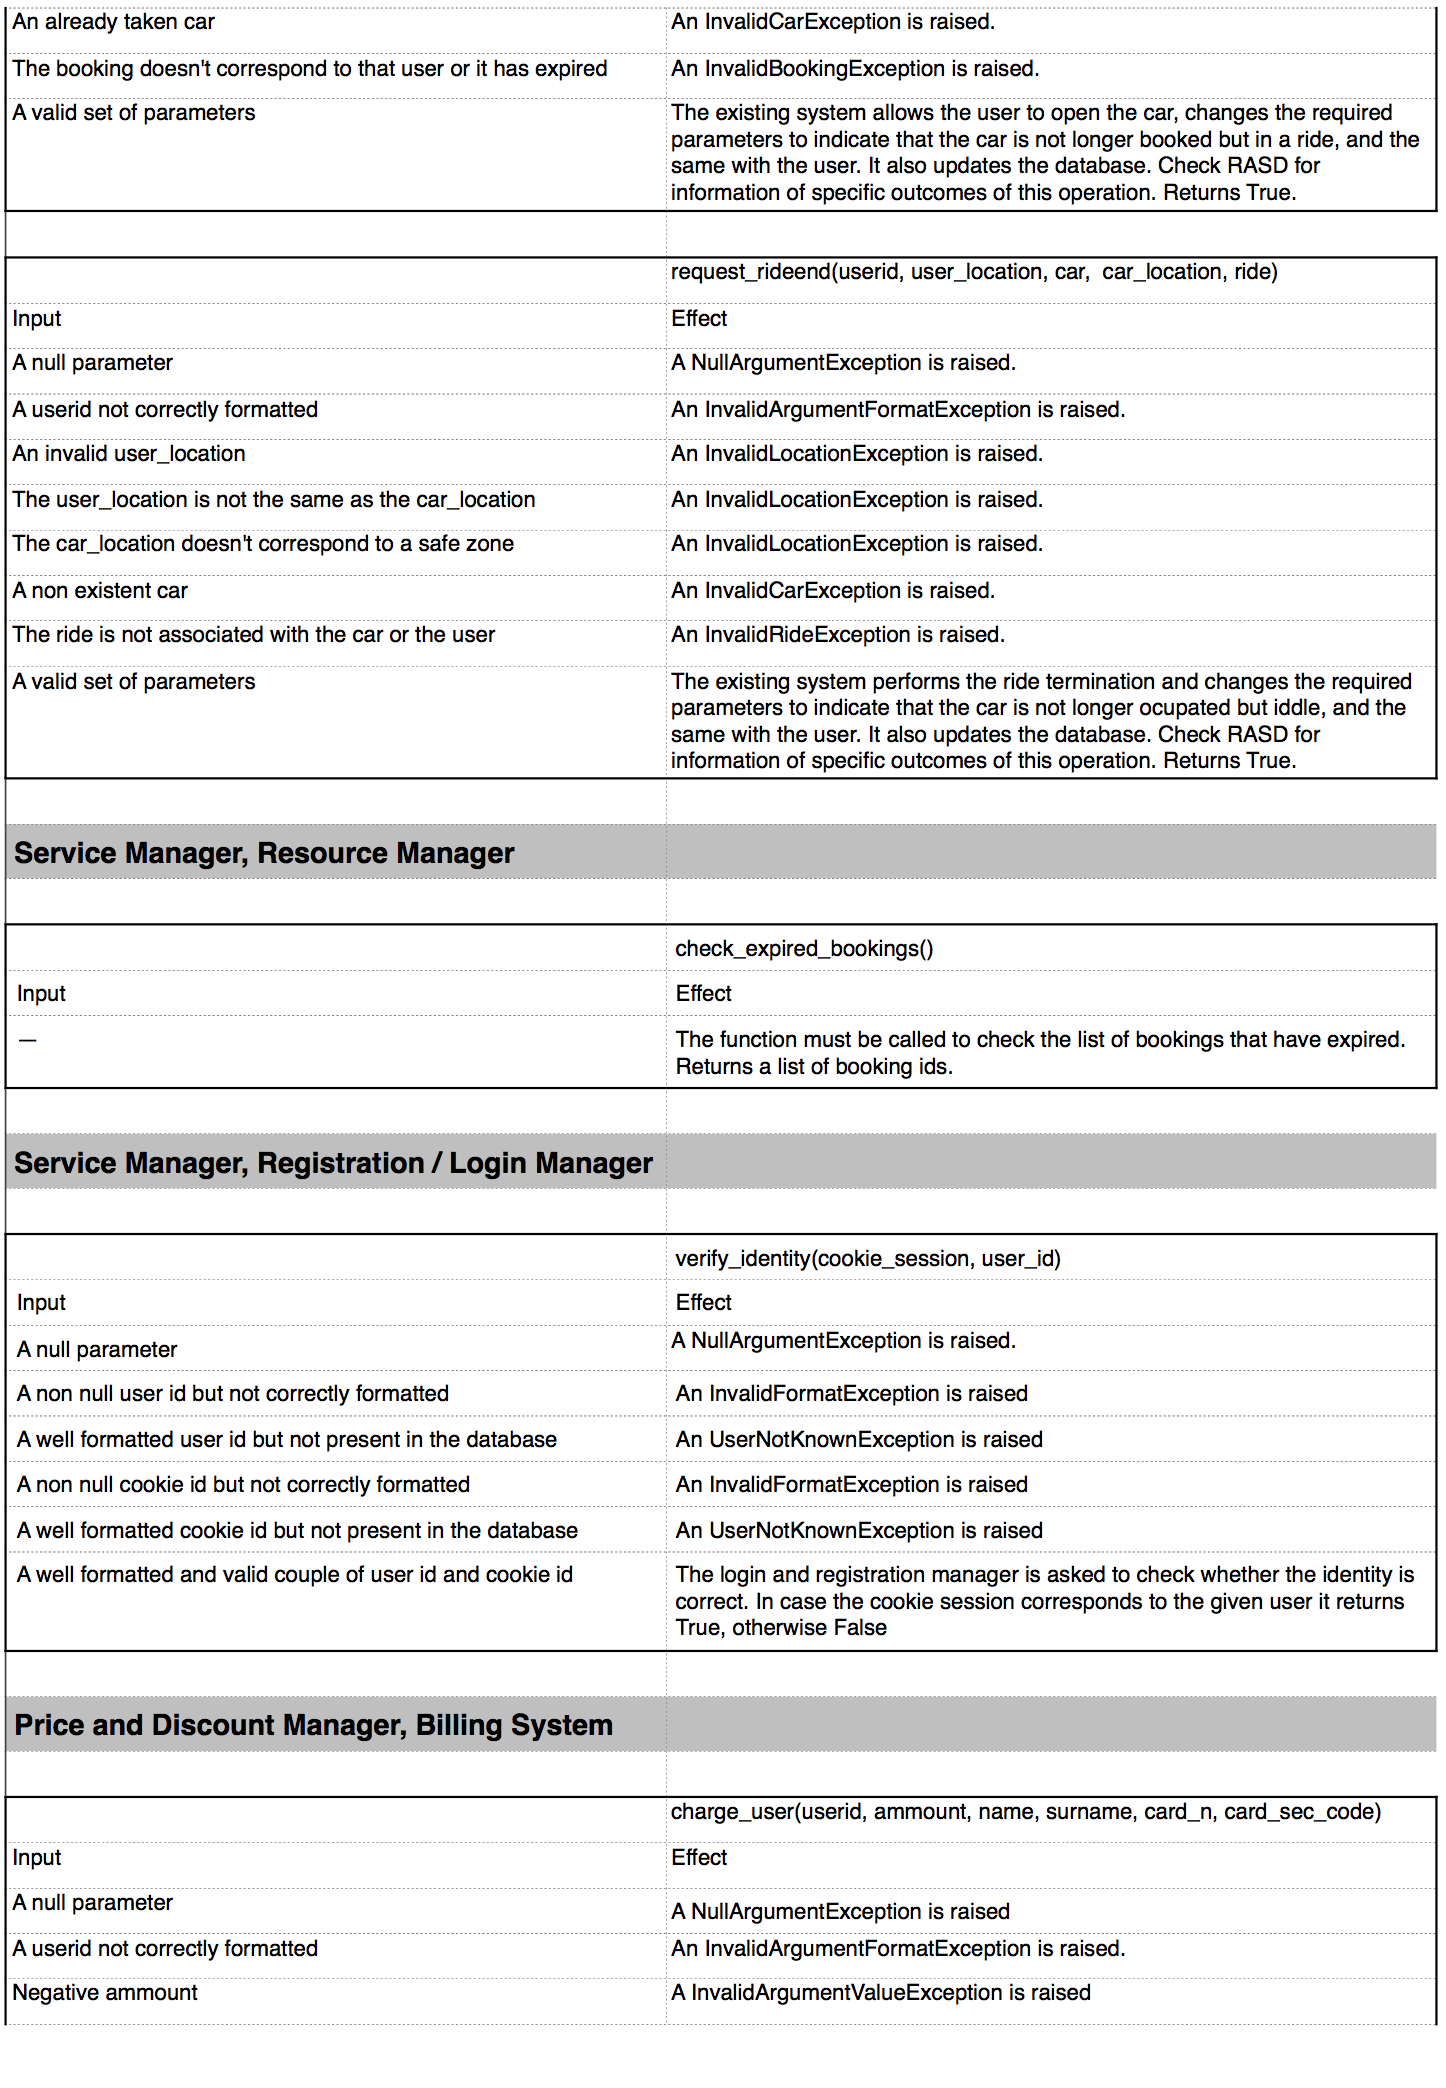
\includegraphics[scale=0.26]{Resources/4.png}
  \end{figure}
    \begin{figure}[!h]
  \centering
    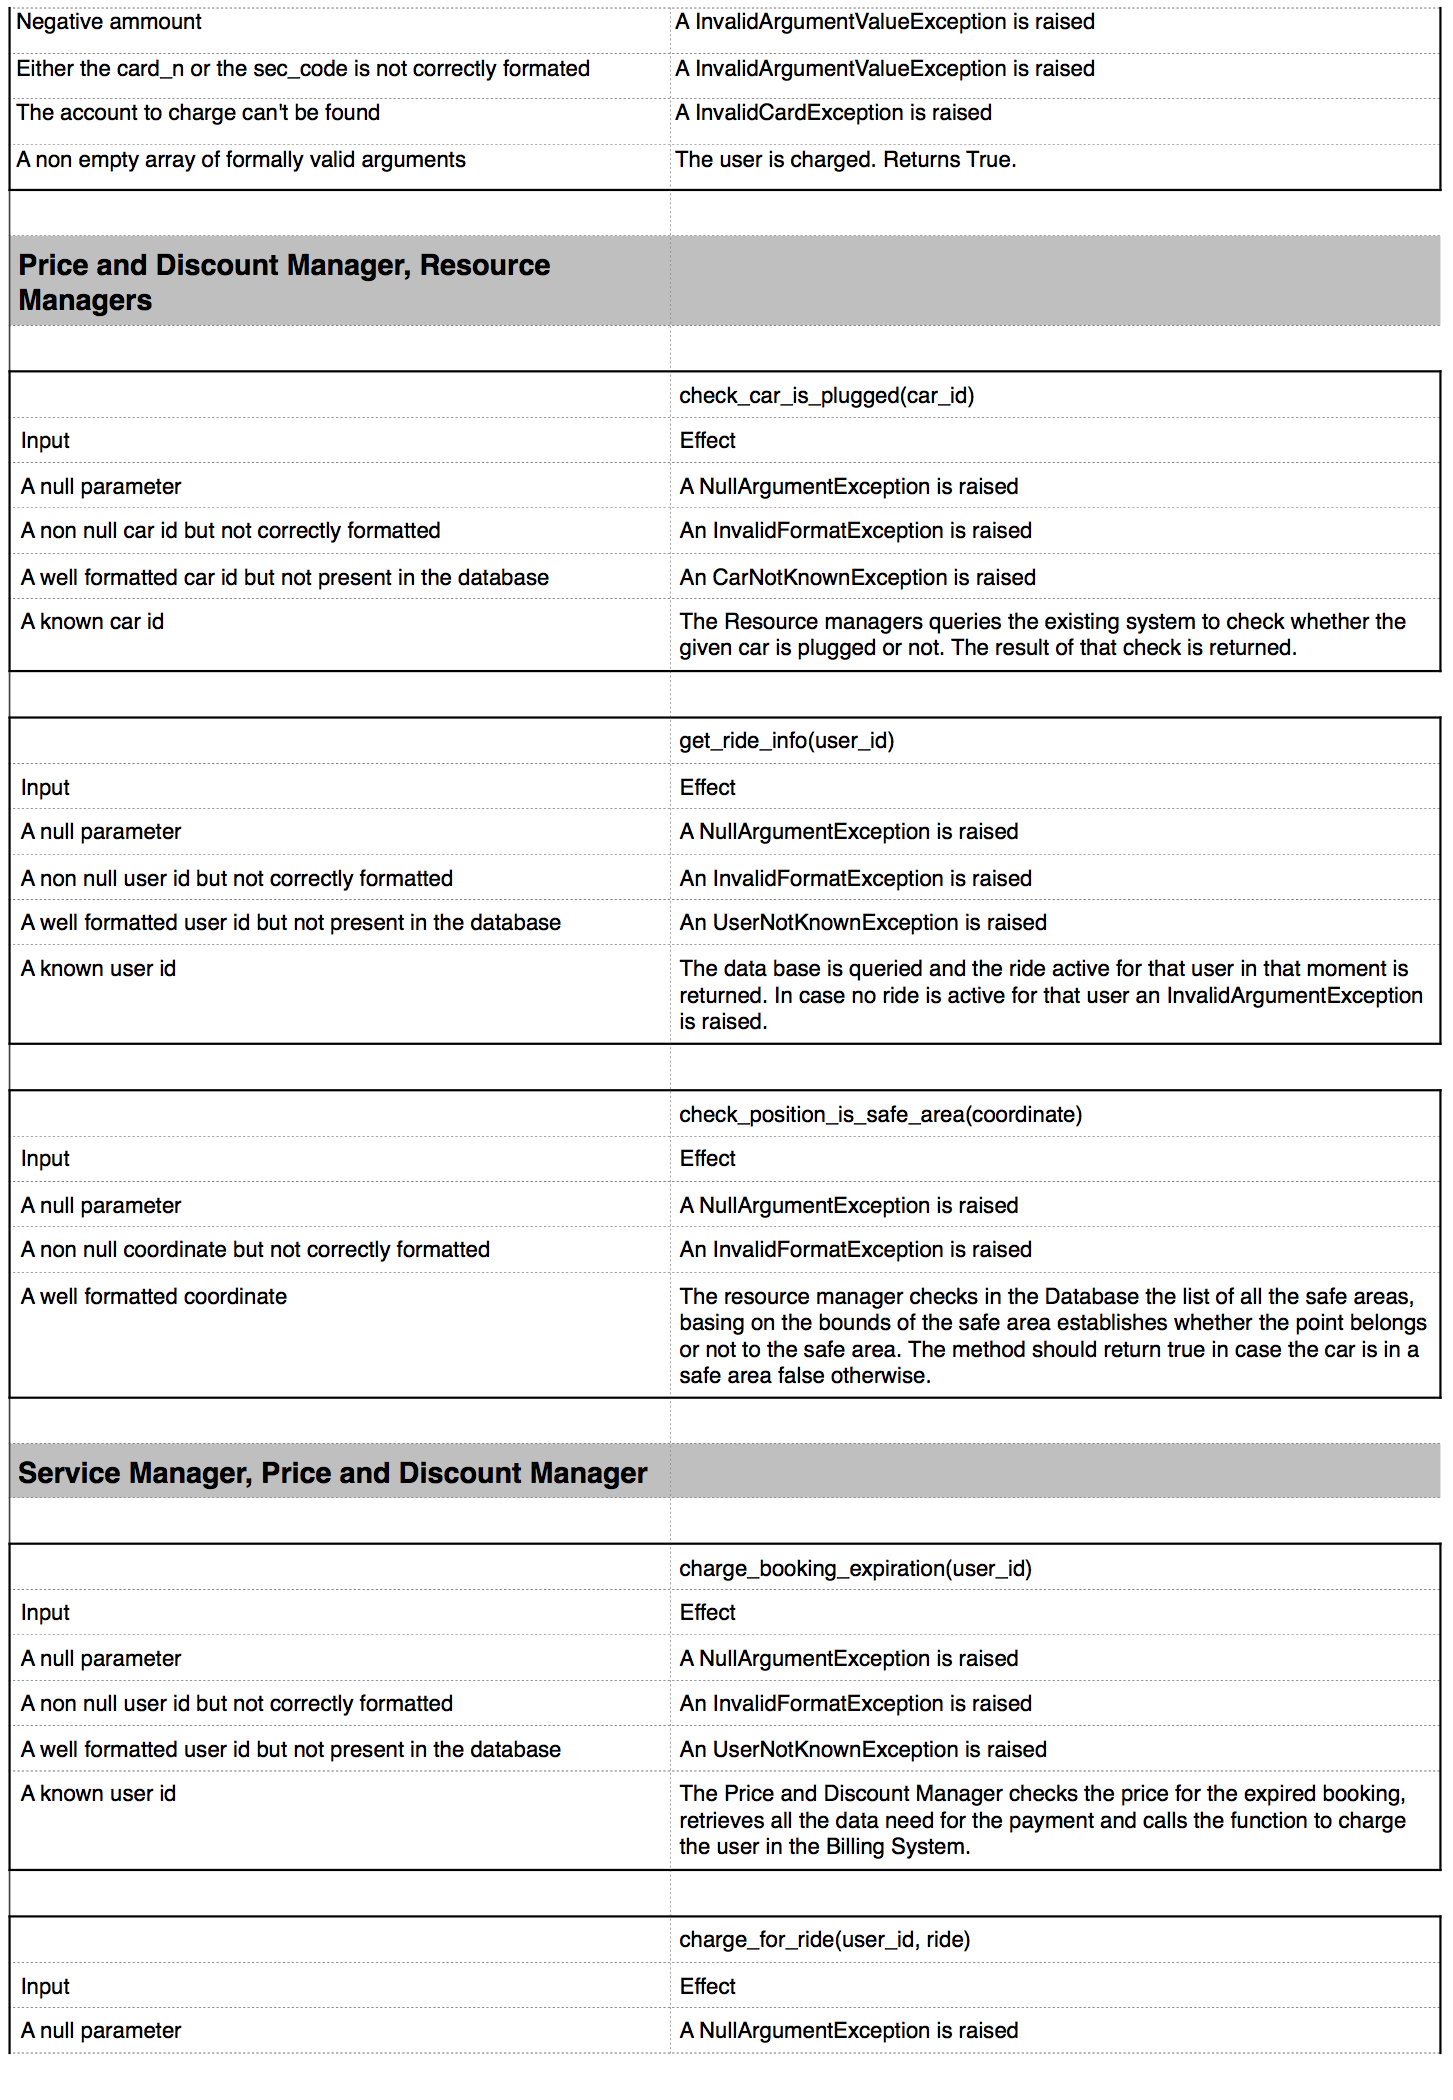
\includegraphics[scale=0.26]{Resources/5.png}
  \end{figure}
    \begin{figure}[!h]
  \centering
    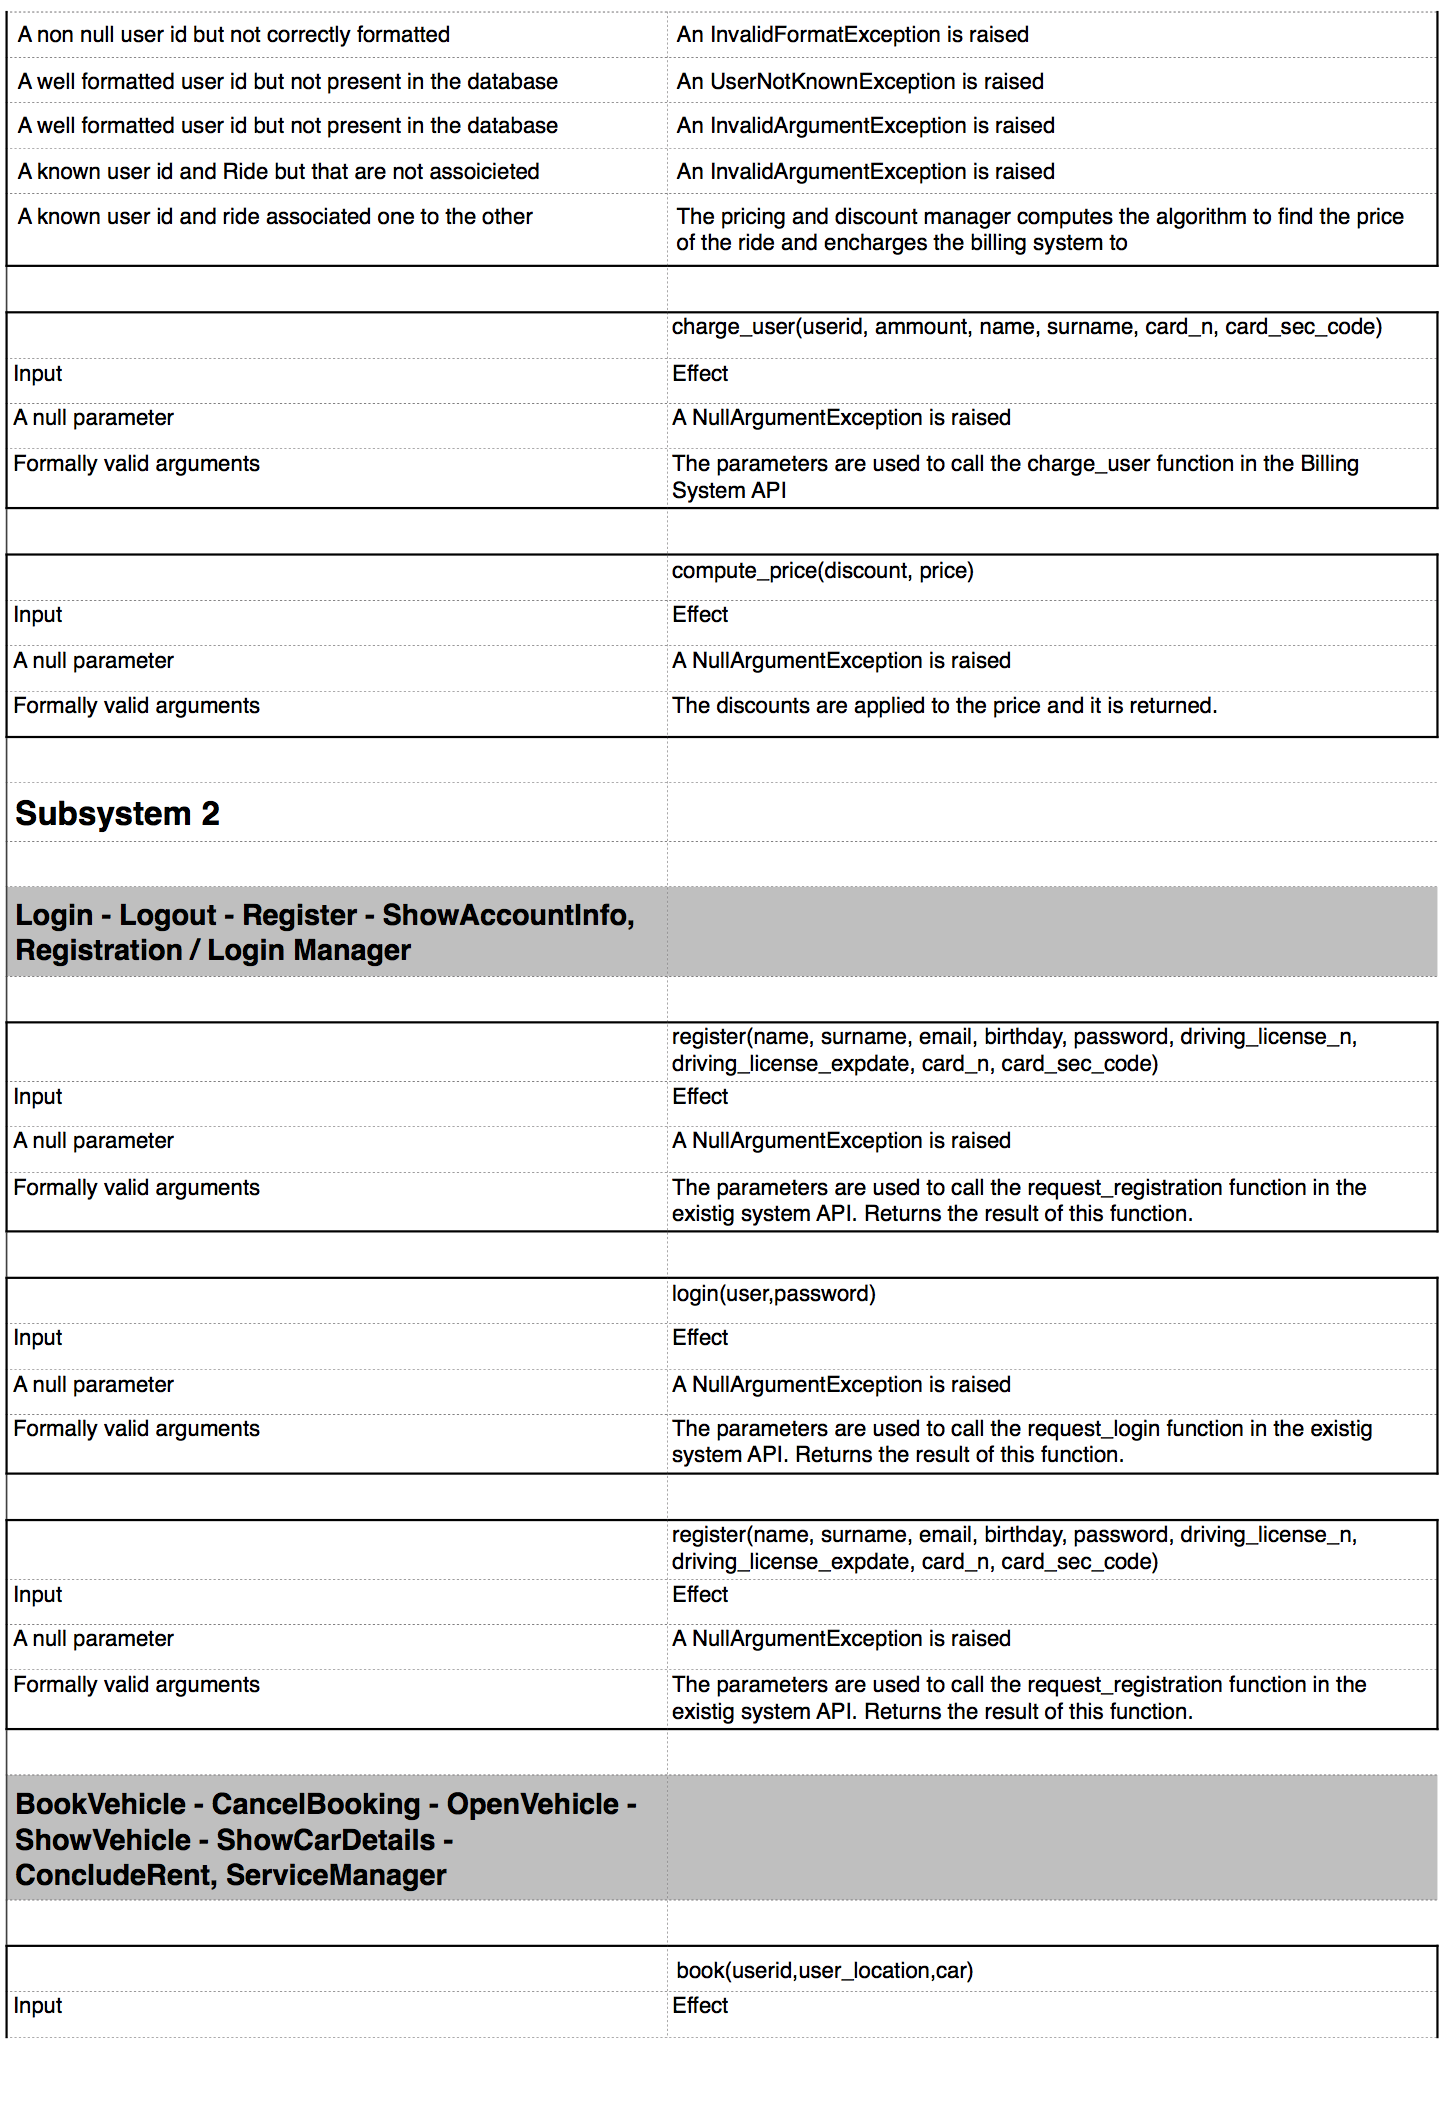
\includegraphics[scale=0.26]{Resources/6.png}
  \end{figure}
    \begin{figure}[!h]
  \centering
    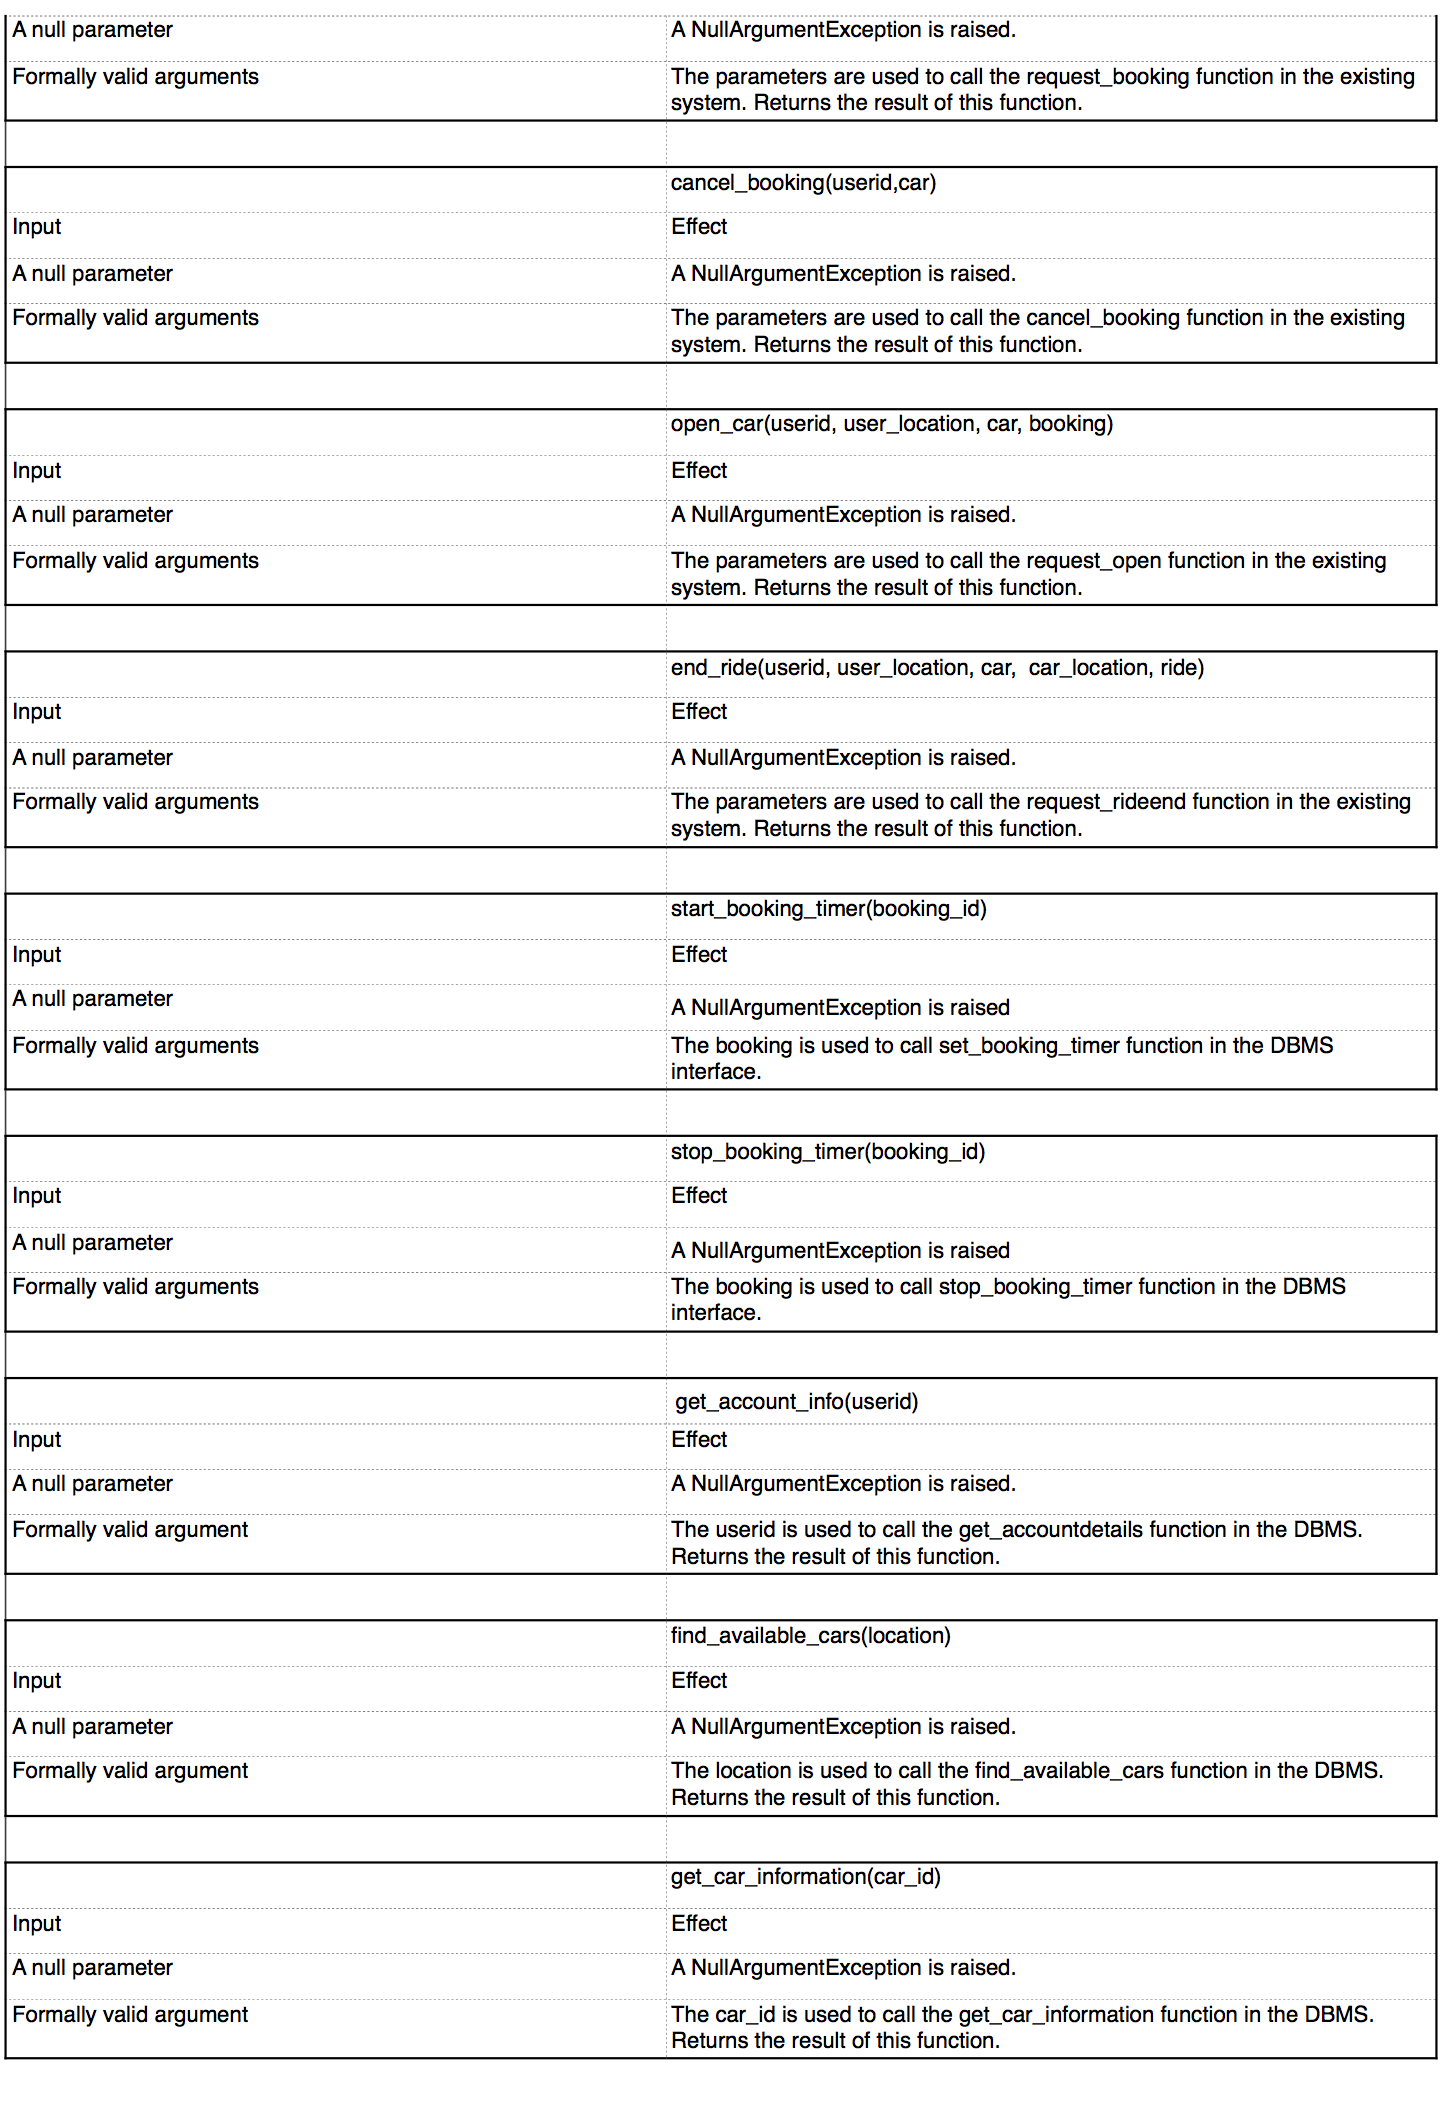
\includegraphics[scale=0.26]{Resources/7.png}
  \end{figure}
    \begin{figure}[!h]
  \centering
    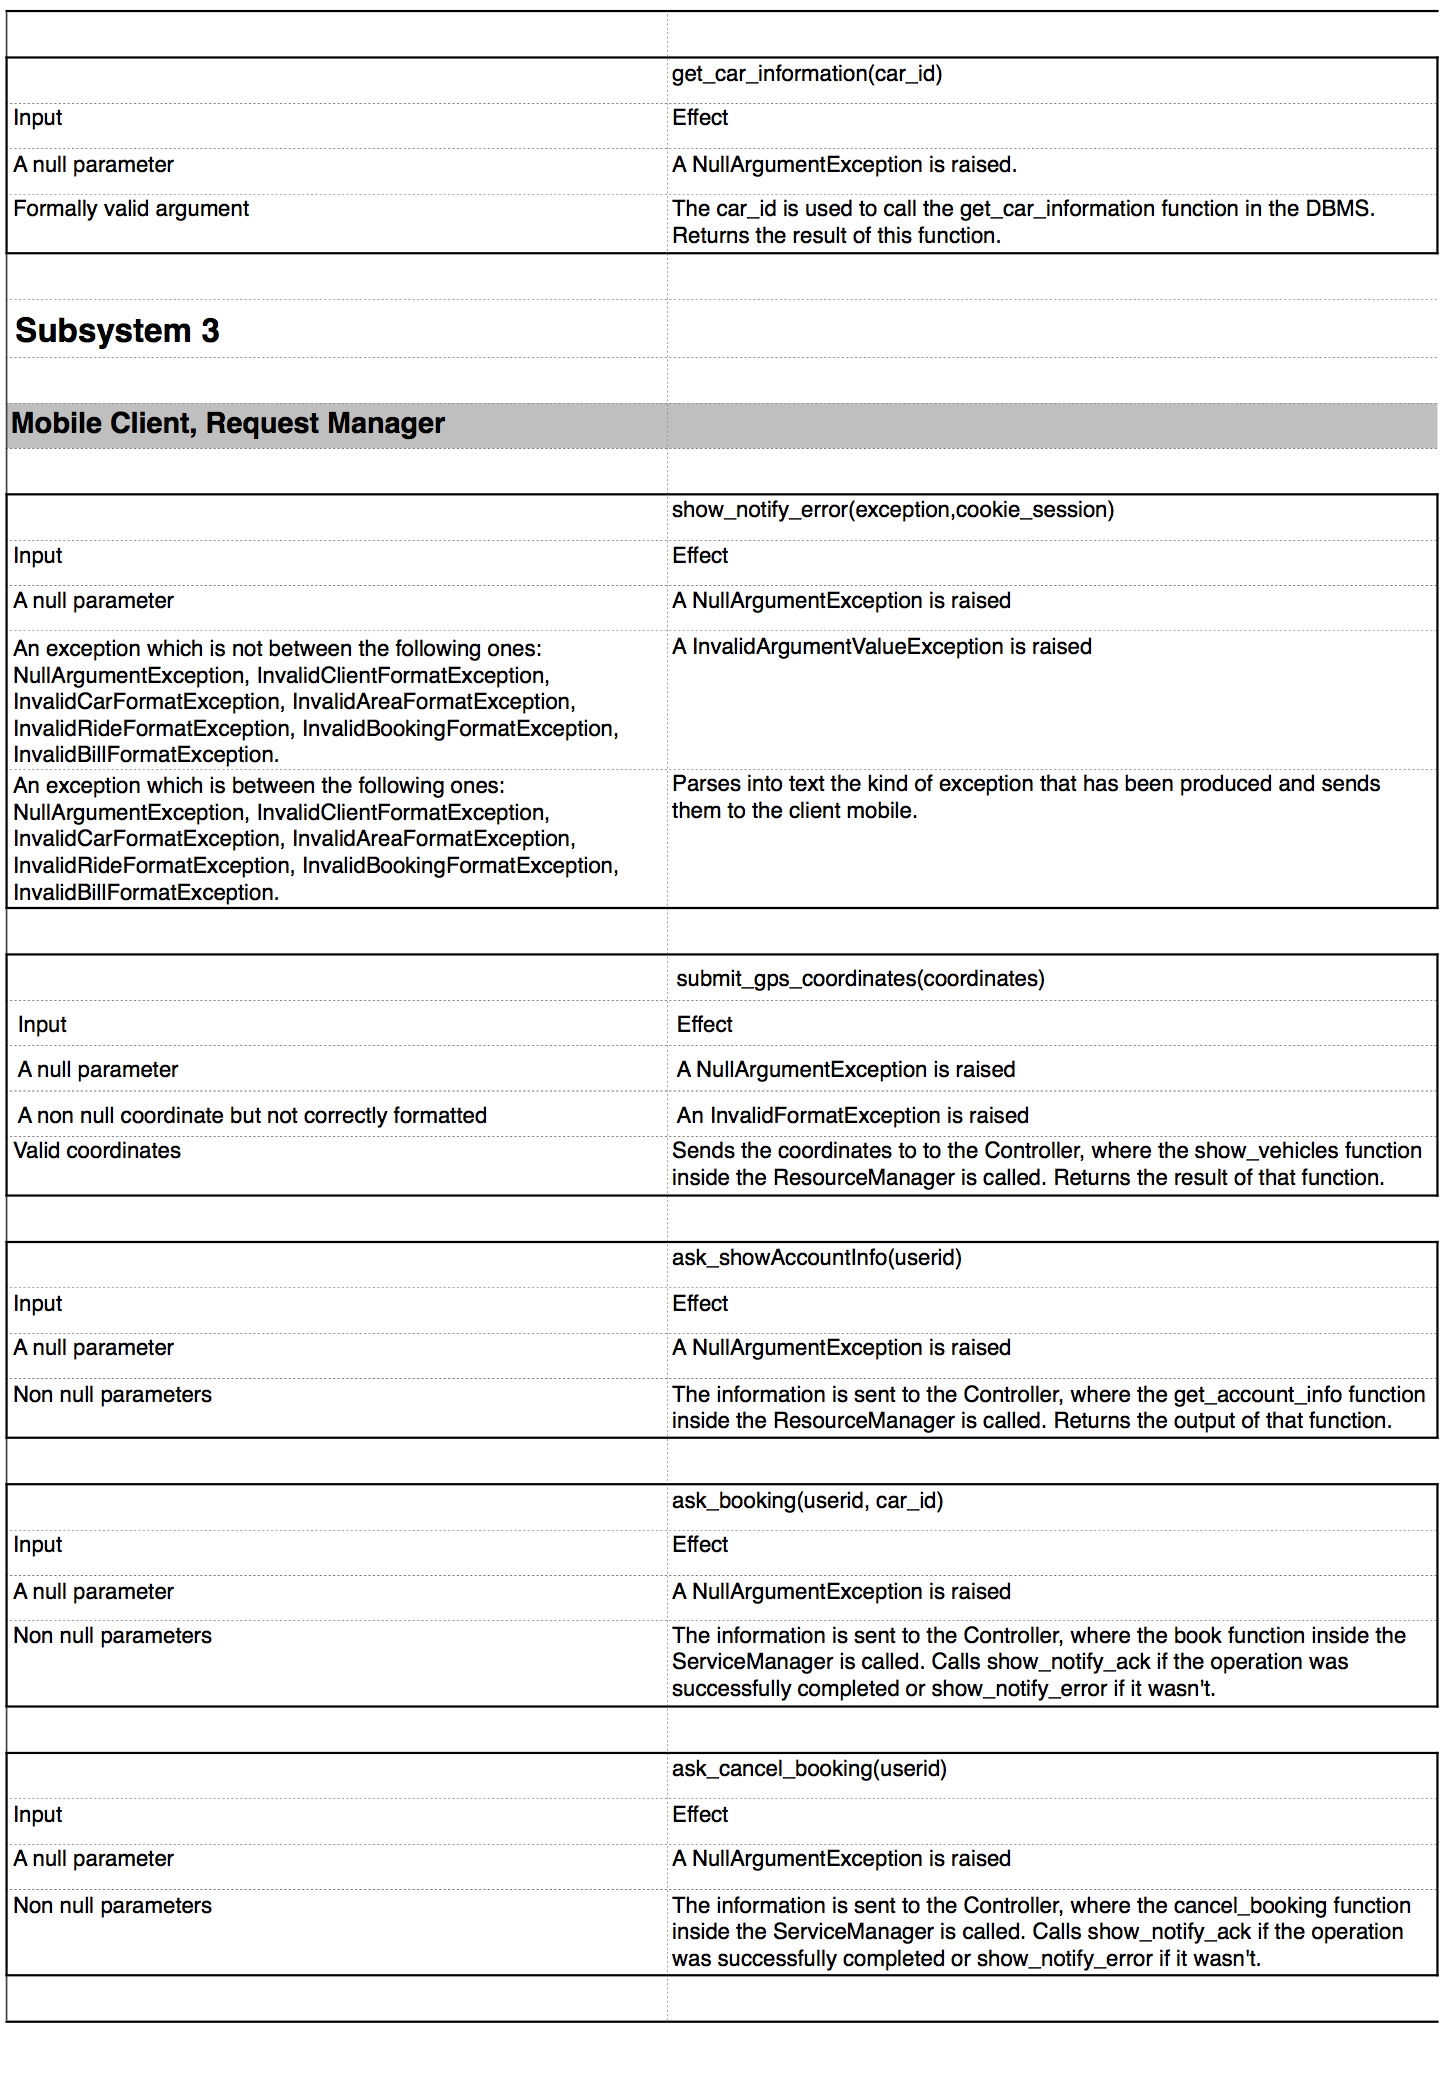
\includegraphics[scale=0.26]{Resources/8.png}
  \end{figure}
    \begin{figure}[!h]
  \centering
    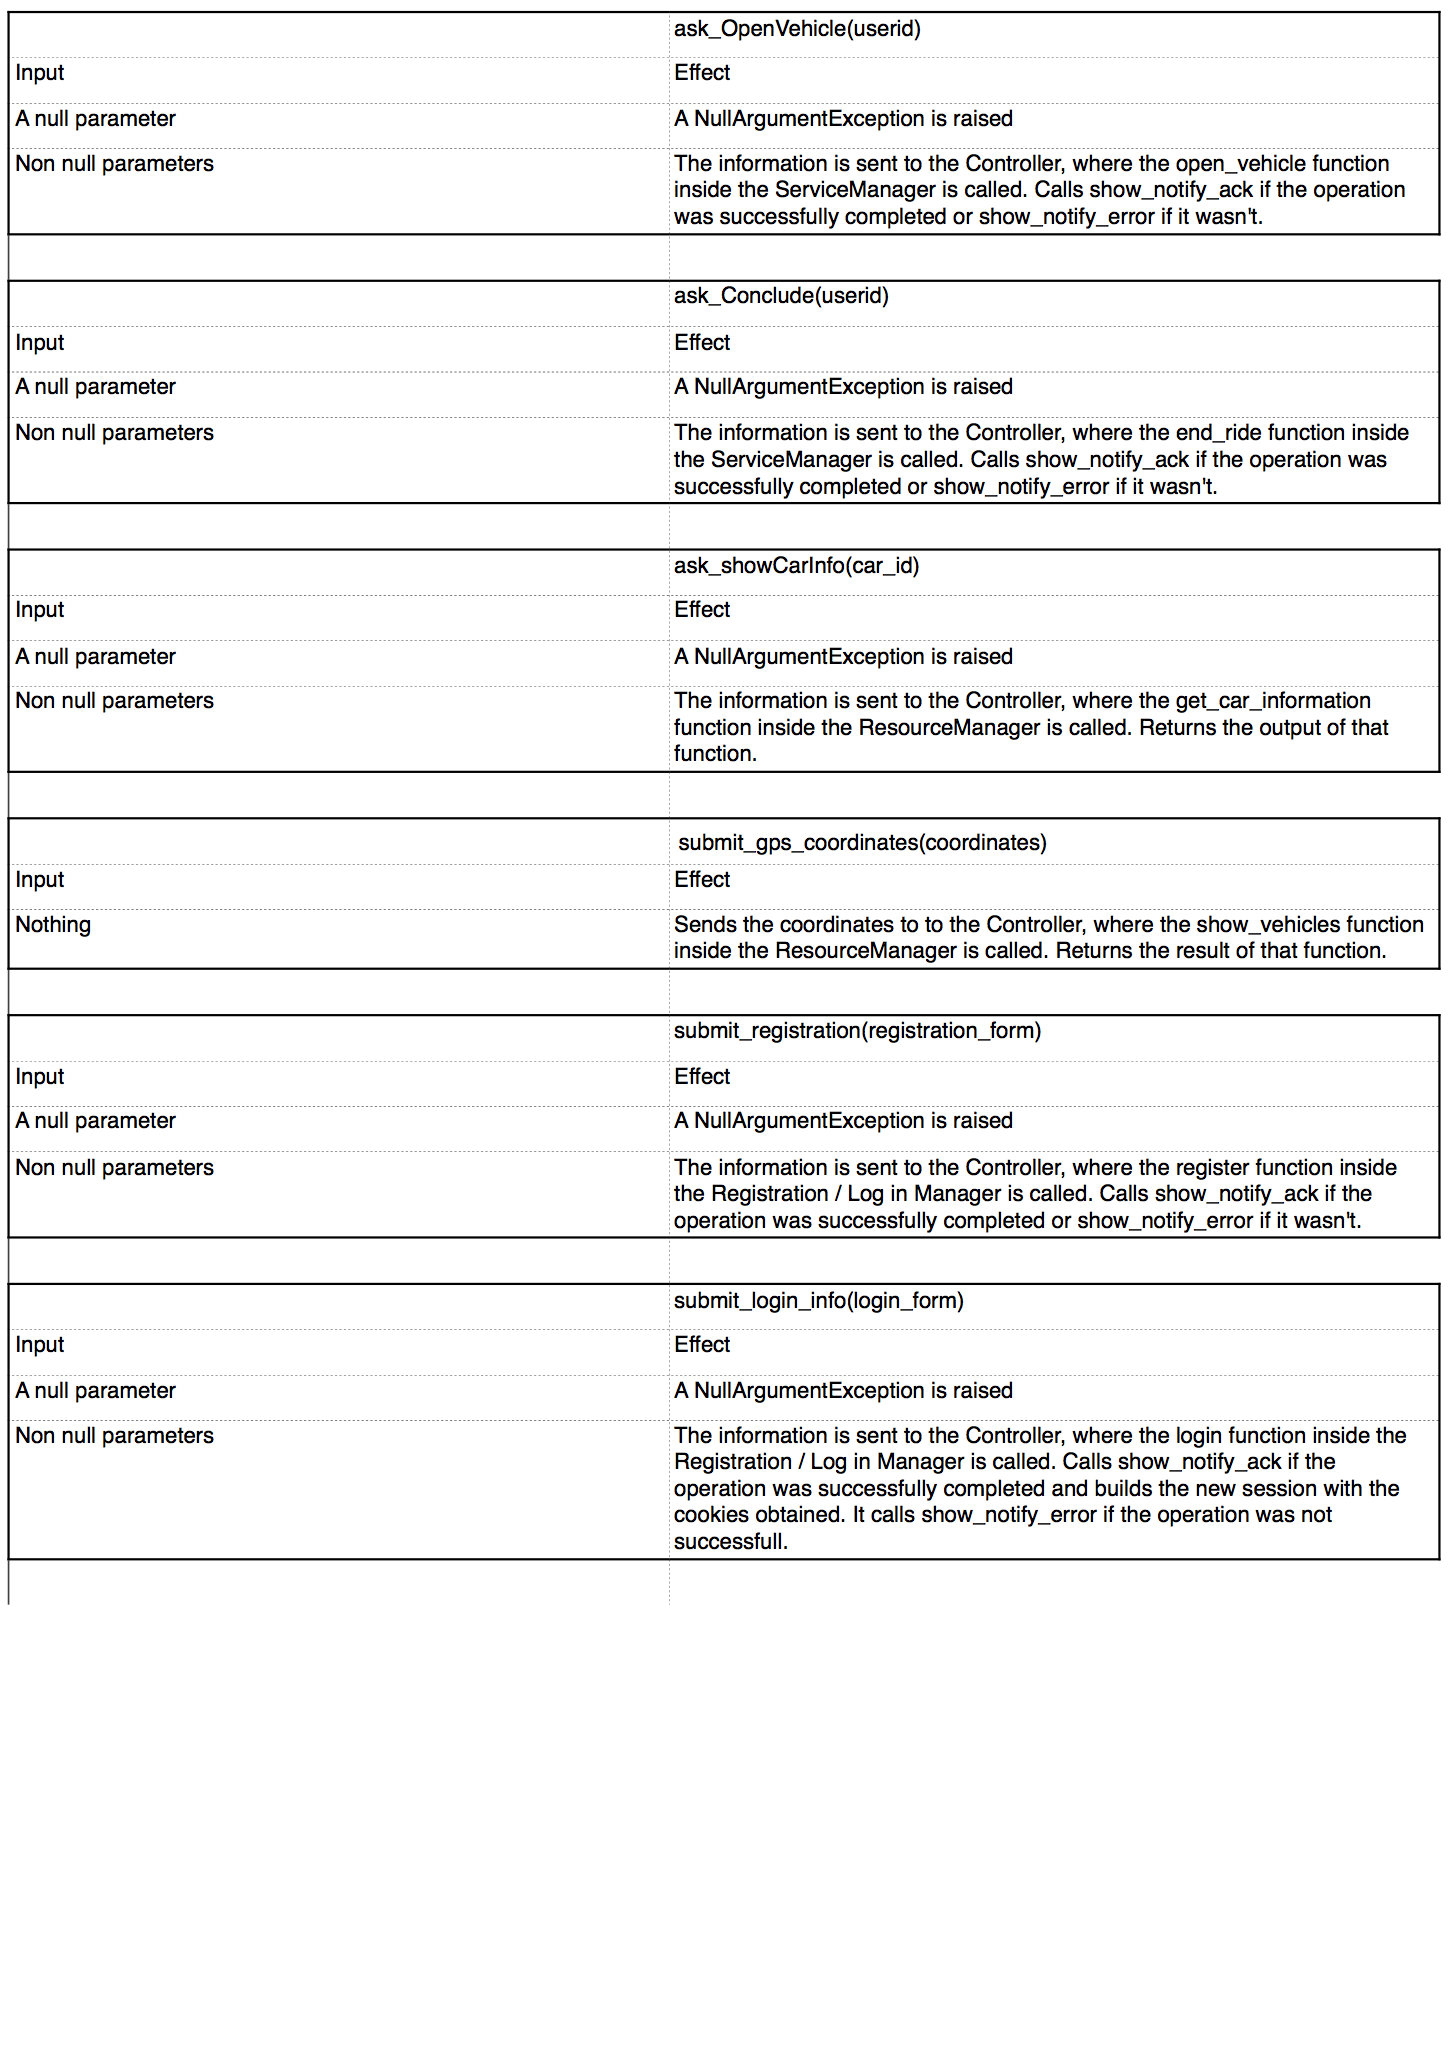
\includegraphics[scale=0.26]{Resources/9.png}
  \end{figure}
  \FloatBarrier
\section{Tools and Required Equipments}

In this section we are going to explain which are the tools that are required to perform the testing activities, why they were selected and how they should be used.
\subsection{Testing Frameworks}
Since the project is written in JEE we are going to exploit two powerfull tools that are designed for Java verification: JUnit and the Arquillion framework. The former, that is 
widely used in unit testing as well, offers the possibility to check that method's calls from one component to the other work in the right way, returning what expected 
and producing the desired effect. The latter, instead, is a tool that is specifically design to support the developer in the integration testing activity and it
can be used in order to verify the correct functioning of the dependency injections and of the interactions of the components between themselves and 
with the database.\\ This two 
components can be considered the main software equipments needed for the testing activity of the control-layer that we have described above. 
For what the customer application is concerned the tools that we are going to use in order to perform the testing activities are the ones that are included in the IDEs used for 
the application development (respectively XCode for iOs and Android Studio for Android).
\subsection{Support Tools}
In some cases the testing activity can be hard or it can fail not because of problems with the code but because of the impossibility to have control on some events 
(e.g.: network's problems). For this reason and in order to be sure that is possible to test also some conditions that appear only rarely we decided to employ Mockito. Mockito
is a testing tool that can allow the developer to define the behaviour of an object and to use the mocked object instead of the real one while testing. In the integration 
testing this can also be usefull because if the behaviour of single units has already been tested and is given for sure. In addition we are going to use GreenMail as a mocked
email service in all those test cases in which an email messaging system is needed. 
\subsection{Testing Equipment} 
The testing activity requires some physical equipments as well. In particular we need one Android device and one iOs device, one web-server where all the business-logic components
are installed and where the mocked version of the Existing System, DBMS and Billing System has been set up.
\end{document}